\documentclass[10pt,a4paper]{article}
\usepackage[utf8]{inputenc}
\usepackage{listings}
\usepackage[english]{babel}
\usepackage{graphicx}
\usepackage[english]{isodate}
\usepackage[parfill]{parskip}


\usepackage{xcolor}

\colorlet{punct}{red!60!black}
\definecolor{background}{HTML}{EEEEEE}
\definecolor{delim}{RGB}{20,105,176}
\colorlet{numb}{magenta!60!black}

\lstdefinelanguage{json}{
    basicstyle=\scriptsize\ttfamily,
    numbers=left,
    numberstyle=\scriptsize,
    stepnumber=1,
    numbersep=8pt,
    showstringspaces=false,
    breaklines=true,
    frame=lines,
    backgroundcolor=\color{background},
    literate=
     *{0}{{{\color{numb}0}}}{1}
      {1}{{{\color{numb}1}}}{1}
      {2}{{{\color{numb}2}}}{1}
      {3}{{{\color{numb}3}}}{1}
      {4}{{{\color{numb}4}}}{1}
      {5}{{{\color{numb}5}}}{1}
      {6}{{{\color{numb}6}}}{1}
      {7}{{{\color{numb}7}}}{1}
      {8}{{{\color{numb}8}}}{1}
      {9}{{{\color{numb}9}}}{1}
      {:}{{{\color{punct}{:}}}}{1}
      {,}{{{\color{punct}{,}}}}{1}
      {\{}{{{\color{delim}{\{}}}}{1}
      {\}}{{{\color{delim}{\}}}}}{1}
      {[}{{{\color{delim}{[}}}}{1}
      {]}{{{\color{delim}{]}}}}{1},
}

\lstdefinelanguage{bash}{
    basicstyle=\normalfont\ttfamily,
    numbers=left,
    numberstyle=\scriptsize,
    stepnumber=10,
    numbersep=8pt,
    showstringspaces=false,
    breaklines=true,
    frame=lines,
    backgroundcolor=\color{background},
    literate=
     *{0}{{{\color{numb}0}}}{1}
      {1}{{{\color{numb}1}}}{1}
      {2}{{{\color{numb}2}}}{1}
      {3}{{{\color{numb}3}}}{1}
      {4}{{{\color{numb}4}}}{1}
      {5}{{{\color{numb}5}}}{1}
      {6}{{{\color{numb}6}}}{1}
      {7}{{{\color{numb}7}}}{1}
      {8}{{{\color{numb}8}}}{1}
      {9}{{{\color{numb}9}}}{1}
      {:}{{{\color{punct}{:}}}}{1}
      {,}{{{\color{punct}{,}}}}{1}
      {\{}{{{\color{delim}{\{}}}}{1}
      {\}}{{{\color{delim}{\}}}}}{1}
      {[}{{{\color{delim}{[}}}}{1}
      {]}{{{\color{delim}{]}}}}{1},
}

\title{TransitMapper Documentation}
\author{Patrick Brosi}

\begin{document}
\maketitle

\section{Usage}

The input file is given as a (simplified) Geo-JSON file, consisting of nodes (represented as ``Point''-features) and edges (represented as ``LineString''-features).

\begin{lstlisting}[language=bash,firstnumber=1]
$ cat input.json | transitmapper -o test.svg
\end{lstlisting}

See below for an example input.

\begin{figure}[htbp]
  \centering
  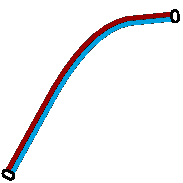
\includegraphics{test.pdf}
  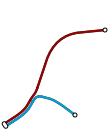
\includegraphics{test2.pdf}
  \caption{Simple example outputs}
\end{figure}

\section{JSON Format}

\section{Example Input}


\begin{lstlisting}[language=json,firstnumber=1]
{
  "type": "FeatureCollection",
  "features": [
    {
      "geometry": {
        "coordinates": [0, 0],
        "type": "Point"
      },
      "properties": {
        "id": "1",
        "station_id": "1"
      }
    },
    {
      "geometry": {
        "coordinates": [1000, 1000],
        "type": "Point"
      },
      "properties": {
        "id": "2",
        "station_id": "2"
      },
      "type": "Feature"
    },
    {
      "geometry": {
        "coordinates": [
          [0, 0], [500, 900], [1000, 950]
        ],
        "type": "LineString"
      },
      "properties": {
        "from": "1",
        "to": "2",
        "lines": [
          {"color": "00a1de"},
          {"color": "990000"}
        ]
      }
    }
  ]
}
\end{lstlisting}
\end{document}